\documentclass{elsarticle}
\usepackage{hyperref}
\usepackage[utf8]{inputenc}
\usepackage{wrapfig}
\usepackage{amsmath}
\usepackage{amsthm}
\usepackage{amssymb}
\usepackage[tmargin=1in,bmargin=1in]{geometry}
\usepackage{caption}
\usepackage{graphicx}
\usepackage{latexsym}
\usepackage{pdfsync}
\usepackage[boxed]{algorithm}
\usepackage{algorithm}
%\usepackage{algpseudocode}
\usepackage{multirow}
\usepackage{rotating}
\usepackage{color}
\usepackage{url}
\usepackage{subfigure}
\usepackage{bigstrut}
\usepackage{bigints}
\usepackage[normalem]{ulem}

\usepackage[normalem]{ulem}




\hypersetup{
    colorlinks=true,              % false: boxed links; true: colored links
    linkcolor=blue,               % color of internal links
    citecolor=blue,               % color of links to bibliography
    filecolor=black,              % color of file links
    urlcolor=red,               % color of external links
    bookmarks=false,
    pdffitwindow=true,
    pdfpagelayout=SinglePage
}

\captionsetup[figure]{font=small,labelfont=normal}

\definecolor{mypink}{cmyk}{0, 0.7808, 0.4429, 0.1412}

\definecolor{mybrown}{cmyk}{0, 0.60, 0.95, 0.63}
\definecolor{darkgreen}{cmyk}{0.98, 0, 0.36, 0.22}


\newcommand{\comment}[1]{\textcolor{red}{[#1]$_{\rm Frederic}$}}
\newcommand{\pouriacomment}[1]{\textcolor{darkgreen}{[#1]$_{\rm Pouria}$}}

\newcommand{\etal}{\textit{et al.\ }}
\newcommand{\pd}[2]{\frac{\partial #1}{\partial #2}}
\newcommand{\mbf}[1]{\mathbf{#1}}
\newcommand{\vect}[1]{\boldsymbol{#1}}
\newcommand{\tensor}[1]{\underline{\underline{\boldsymbol{#1}}}}
\newcommand{\mat}[1]{\underline{\underline{\boldsymbol{#1}}}}
\newcommand{\be}{\begin{equation}}
\newcommand{\ee}{\end{equation}}
\newcommand{\ben}{\begin{equation*}}
\newcommand{\een}{\end{equation*}}
\newcommand{\bea}{\begin{eqnarray}}
\newcommand{\eea}{\end{eqnarray}}
\newcommand{\bean}{\begin{eqnarray*}}
\newcommand{\eean}{\end{eqnarray*}}

\newcommand{\fphi}[2]{\frac{\phi_#1}{\phi_#1-\phi_#2}}
\newcommand{\lif}[2]{\frac{f_#1\phi_#2-f_#2\phi_#1}{\phi_#2-\phi_#1}}
\newcommand{\dx}{{\Delta x}}
\newcommand{\dy}{{\Delta y}}
\newcommand{\dz}{{\Delta z}}
\newcommand{\dt}{{\Delta t}}
\newcommand{\hf}{{\frac12}}
\newcommand{\U}{\vect{U}}
\newcommand{\n}{\vect{n}}



\usepackage{algorithm}
\usepackage[noend]{algpseudocode}
\makeatletter
\def\BState{\State\hskip-\ALG@thistlm}
\makeatother



\begin{document}
\title{JAX-DIPS: Differentiable Interfacial PDE Solver}

\cortext[cor]{Corresponding author: p.a.mistani@gmail.com}


\author[1]{Pouria A. Mistani\thanks{corresponding author} $^{\dagger,}$}
\author[2]{Samira Pakravan$^{\dagger,}$}
\author[1]{Rajesh Ilango}
\author[2]{Frederic G. Gibou}

\address[1]{NVIDIA Corporation, Santa Clara, CA 95051, USA}
\address[2]{University of California, Santa Barbara, CA 93106-5070, USA}

\begin{abstract}
	We present an end-to-end differentiable PDE solver supporting both forward and inverse free boundary problems using the level-set method. We implemented this framework using JAX, extending support for CPU/GPU/TPU platforms. Algorithmically, our proposed framework builds on the blended inverse PDE solver architecure (BiPDE) that authors have proposed earlier \cite{pakravan2021solving}. JAX-DIPS is an open-source software package published under MIT license and is available at \href{https://github.com/JAX-DIPS/JAX-DIPS}{https://github.com/JAX-DIPS/JAX-DIPS}.

\end{abstract}

\begin{keyword}
	level-set method \sep free boundary problems \sep inverse problems \sep jump conditions \sep differentiable programming
\end{keyword}

\maketitle
\def\thefootnote{$\dagger$}\footnotetext{These authors contributed equally to this work}







%%%%%%%%%%%%%%%%%%%%%%%%%%%%%%%%%%%%%
%%%%%%%%%%%%%%%%%%%%%%%%%%%%%%%%%%%%%
\section{Introduction}
\label{sec::introduction}
Differentiable programming ...

DTO vs OTD: we are doing DTO which is Discretize then Optimize paradigm. OTD is the traditional adjoint methods.

JAX-DIPS Poisson problem solver provides the two sides of $A u =b$ which is obtained after discretization of the governing PDE problem over a uniform 3D grid. Two solution schemes for the forwards problem are possible: (1) using usual iterative methods having left-hand-side and right-hand-side of the PDE discretization, and (2) using autodifferentiation across loss function (difference between lhs and rhs in 2-norm) with respect to a given estimate for the solution vector on the underlying grid $\rm u_{ijk}$. Both approaches focus on minimizing the residual over the grid points
\begin{align*}
	\min_{u_{ijk}} \vert\vert Au -b \vert \vert^2_2
\end{align*}
The first method attempts to span the residual space in an iterative fashion by \textit{estimating} the gradient of the minimizing function, while the second method offered in JAX-DIPS is directly computing the exact gradient of the minimizing function with respect to the current estimate for solution. Therefore, the advantage of this method is fewer iterations and faster convergence specially for irregular geometries where the condition number of the linear system leads to much difficulties that need to be resolved by complex preconditioning and increased number of iterations.



\section{Numerical Scheme for Free Boundary Problems}
Consider a closed irregular interface ($\rm \Gamma$) that partitions the computational domain ($\rm \Omega$) into interior ($\rm \Omega^-$) and exterior ($\rm \Omega^+$) subdomains; \textit{i.e.}, $\rm \Omega=\Omega^- \cup \Gamma \cup \Omega^+$. We are interested in the solutions $\rm u^\pm\in \Omega^\pm$ to the following class of linear elliptic problems in  $\rm \mathbf{x}\in\Omega^\pm$:
\begin{align*}
	 & k^{\pm}u^{\pm} - \nabla \cdot (\mu^{\pm}\nabla u^\pm)=f^{\pm}, & \mathbf{x}\in\Omega^\pm \\
	 & [u]=\alpha,                                                    & \mathbf{x} \in \Gamma   \\
	 & [\mu \partial_{\mathbf{n}}u]=\beta,                            & \mathbf{x} \in \Gamma
\end{align*}
Here $f^\pm=f(\mathbf{x} \in \Omega^\pm)$ is the spatially varying source term, $\rm \mu^\pm=\mu(\mathbf{x} \in \Omega^\pm)$  are the diffusion coefficients, and $k^\pm$ are the reaction coefficients in the two domains. We consider Dirichlet boundary conditions in a cubic domain $\rm \Omega=[-L/2,L/2]^3$.


\subsection{The level-set method}

\subsection{Finite discretization method}

For spatial discretizations at the presence of jump conditions we employ the numerical algorithm proposed by Bochkov and Gibou (2020) \cite{bochkov2020solving} (BG20) on Cartesian grids. BG20 produces second-order accurate solutions and first-order accuracte gradients in the $L^\infty$-norm, while having a compact stencil that makes it a good candidate for parallelization. Moreover, treatment of the interface jump conditions do not introduce any augmented variables, this preserves the homogeneous structure of the linear system.

Here we use a finite volume discretization equation uniformly for all grid points. At grid points where the finite volumes are crossed by $\rm \Gamma$ we have

\begin{align*}
	 & \sum_{s=-,+}\int_{\Omega^s \cap \mathcal{V}_{i,j}}  k^{s} u^{s} d\Omega -\sum_{s=-,+} \int_{\Omega^s\cap \partial\mathcal{V}_{i,j}} \mu^{s}\partial_{\mathbf{n}^s} u^s  d\Gamma = \sum_{s=-,+}\int_{\Omega^s \cap \mathcal{V}_{i,j}}  f^{s} d\Omega + \int_{\Gamma \cap \mathcal{V}_{i,j}}[\mu\partial_{\mathbf{n}}u]d\Gamma \\
	\intertext{following standard treatment of volumetric integrals and using central differencing for derivatives we obtain in 2D (with trivial 3D extension)}
	 & \sum_{s=-,+} k_{i,j}^s u_{i,j}^{s} |\mathcal{V}_{i,j}^s| - \sum_{s=-,+}\bigg( \mu_{i-\frac{1}{2},j}^s A_{i-\frac{1}{2},j}^s\frac{u_{i-1,j}^s - u_{i,j}^s}{\Delta x}     +   \mu_{i+\frac{1}{2},j}^s A_{i+\frac{1}{2},j}^s\frac{u_{i+1,j}^s - u_{i,j}^s}{\Delta x} +                                                          \\
	 & \mu_{i, j-\frac{1}{2}}^s A_{i, j-\frac{1}{2}}^s\frac{u_{i,j-1}^s - u_{i,j}^s}{\Delta y} + \mu_{i, j+\frac{1}{2}}^s A_{i, j+\frac{1}{2}}^s\frac{u_{i,j+1}^s - u_{i,j}^s}{\Delta y} \bigg)                                                                                                                                     \\
	 & =  \sum_{s=-,+} f_{i,j}^{s} |\mathcal{V}_{i,j}^s| + \int_{\Gamma\cap \mathcal{V}_{i,j}} \beta d\Gamma + \mathcal{O}(\max(\Delta x, \Delta y)^\mathcal{D})
\end{align*}
where $\mathcal{D}$ is the problem dimensionality.

\begin{figure}
	\centering
	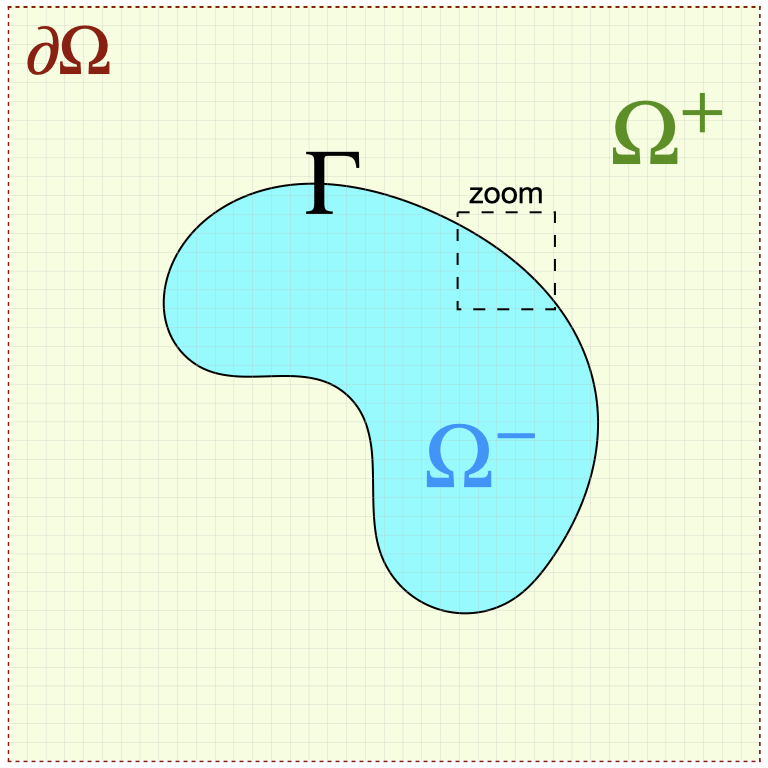
\includegraphics[width=0.45\linewidth]{./figures/grids_full.png}
	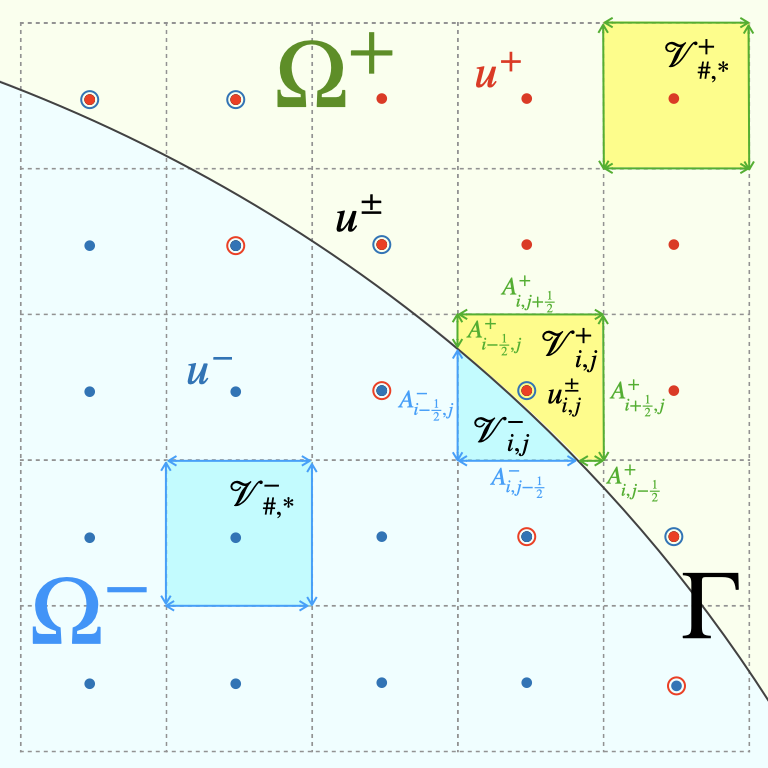
\includegraphics[width=0.45\linewidth]{./figures/grids.png}
	\caption{Notation used in this paper. Close to the interface where finite volumes are crossed by the interface, there are extra degrees of freedom (open circles) that are extrapolations of solutions from each domain to the opposite domain. Jump conditions are implicitly encoded in these extrapolated values.}
	\label{fig:grid}
\end{figure}

Note that far from interface either $s=-$ (for $\mathbf{x}\in \Omega^-$) or $s=+$ (for $\mathbf{x}\in \Omega^+$) is retained. This is automatically considered through zero values for sub-volumes $|\mathcal{V}_{i,j}^+|$ and $|\mathcal{V}_{i,j}^-|$ as well as their face areas. Note that $\mu_{i-1/2,j}^-$ (or $\mu_{i-1/2,j}^+$) corresponds to the value of diffusion coefficient at the middle of segment $A^-_{i-1/2,j}$ (or $A^+_{i-1/2,j}$) respectively, same is true for other edges as well. However, there are extra degrees of freedom on grid points whose finite volumes are crossed by the interface; \textit{i.e.}, see double circles in figure \ref{fig:grid}. Bochkov and Gibou derived analytical expressions for the extra degrees of freedom ($u^+$ in $\Omega^-$ and $u^-$ in $\Omega^+$) in terms of the original degrees of freedom ($u^-$ in $\Omega^-$ and $u^+$ in $\Omega^+$) as well as the jump conditions, this preserves the original $\rm N_x \times N_y$ system size.

In this scheme the basic idea is to extrapolate the jump at grid point from jump condition at the projected point onto the interface using a Taylor expansion: $u^+_{i,j} - u^-_{i,j}=[u]_{\mathbf{r}_{i,j}^{pr}} + \delta_{i,j}(\partial_\mathbf{n}u^+(\mathbf{r}^{pr}_{i,j}) - \partial_\mathbf{n}u^-(\mathbf{r}^{pr}_{i,j})) $. The unknown value ($u^-_{i,j}$ or $u^+_{i,j}$) is obtained based on approximation of the normal derivatives (\textit{i.e.} $\partial_\mathbf{n}u^\pm(\mathbf{r}^{pr}_{i,j})$) which are computed using a least squares calculation on neighboring grid points that are in the fast-diffusion region (referred to as ``Bias Fast'') or in the slow diffusion region (referred to as ``Bias Slow''). This makes two sets of ruls for unknown values $u^\pm_{i,j}$.

In two dimensions and on uniform grids, the gradient operator at the grid cell $(i,j)$ that is crossed by an interface is estimated by a least squares solution given by
\begin{align*}
	 & (\nabla u^\pm)_{i,j} = \mathbf{D}^\pm_{i,j} \begin{bmatrix}
		u_{i-1,j-1} - u^\pm_{i,j} \\
		u_{i,j-1} - u^\pm_{i,j}   \\
		\vdots                    \\
		u_{i+1,j+1} - u^\pm_{i,j}
	\end{bmatrix} & \mathbf{D}^\pm_{i,j} = \big(X^T_{i,j} W^\pm_{i,j} X_{i,j} \big)^{-1} \big( W^\pm_{i,j} X_{i,j} \big)^T
\end{align*}
and
\begin{align*}
	 & W^\pm_{i,j} = \begin{bmatrix}
		 & \omega^\pm_{i,j} (-1,-1) &                         &        &                        \\
		 &                          & \omega^\pm_{i,j} (0,-1) &        &                        \\
		 &                          &                         & \ddots &                        \\
		 &                          &                         &        & \omega^\pm_{i,j} (1,1) \\
	\end{bmatrix} & X_{i,j} = \begin{bmatrix}
		 & -h_x & -h_y \\
		 & 0    & -h_y \\
		 & h_x  & -h_y \\
		 & -h_x & 0    \\
		 & 0    & 0    \\
		 & h_x  & 0    \\
		 & -h_x & h_y  \\
		 & 0    & h_y  \\
		 & h_x  & h_y
	\end{bmatrix}
\end{align*}
and
\begin{equation}
	\omega_{i,j}^\pm (p,q) = \begin{cases}
		1 & (p,q)\in N_{i,j}^\pm \\
		0 & \text{else}
	\end{cases}
\end{equation}
In this case, $D^\pm_{i,j}$ is a $2\times 9$ matrix and we denote each of its $2\times 1$ columns with $d^\pm_{i,j,p,q}$
\begin{align*}
	\mathbf{D}^\pm_{i,j}  = \begin{bmatrix}
		 & d^\pm_{i,j,-1,-1} & d^\pm_{i,j,0,-1} & d^\pm_{i,j,1,-1} & d^\pm_{i,j,-1,0} & d^\pm_{i,j,0,0} & d^\pm_{i,j,1,0} & d^\pm_{i,j,-1,1} & d^\pm_{i,j,0,1} & d^\pm_{i,j,1,1}
	\end{bmatrix}
\end{align*}
The least square coefficients are then obtained by dot product of normal vector with these columns
\begin{align*}
	c^\pm_{i,j,p,q} = \mathbf{n}_{i,j}^T  d^\pm_{i,j,p,q}
\end{align*}
At this point we can define a few intermediate variables at each grid point to simplify the presentation of the method,
\begin{align*}
	 & \zeta_{i,j,p,q}^\pm := \delta_{i,j} \frac{[\mu]}{\mu^\mp}c_{i,j,p,q}^\pm  & \zeta_{i,j}^\pm := -\sum_{(p,q)\in N_{i,j}^\pm} \zeta_{i,j,p,q}^\pm   \\
	 & \gamma_{i,j,p,q}^\pm := \frac{\zeta_{i,j,p,q}^\pm}{1 \pm \zeta^\pm_{i,j}} & \gamma^\pm_{i,j} := -\sum_{(p,q)\in N_{i,j}^\pm} \gamma_{i,j,p,q}^\pm
\end{align*}
where the set of neighboring grid points are
\begin{align*}
	N_{i,j}^\pm = \{(p,q) :\ \ \  p=-1,0,1, \ \ \  q=-1,0,1, \ \ \ (p,q)\neq (0,0), \ \ \ \mathbf{x}_{i+p,j+q}\in \Omega^\pm \}
\end{align*}
and $\delta_{i,j}$ is the signed distance from $\mathbf{x}_{i,j}$ that is computed from the level-set function $\phi(\mathbf{x})$
\begin{align*}
	\delta_{i,j}=\frac{\phi(\mathbf{x}_{i,j})}{|\nabla \phi(\mathbf{x}_{i,j})|}
\end{align*}

\begin{itemize}
	\item Rules based on approximating $\partial_\mathbf{n}u^+(\mathbf{r}^{pr}_{i,j})$:
\end{itemize}
%\begin{equation}
% u_{i,j}^-=\begin{cases}
%    u_{i,j}, & \text{ $\mathbf{x}_{i,j}\in \Omega^-$}\\
%    u_{i,j} - \alpha_1 -\delta_{i,j}\frac{\beta_1}{\mu^{+}} - \delta_{i,j} \frac{[\mu]}{\mu^+} \bigg( \frac{ c_{i,j}^- (u_{i,j} - \alpha_1 - \delta_{i,j}\frac{\beta_1}{\mu^+}) + \sum_{(p,q)\in N_{i,j}^-} c_{i,j,p,q}^- u_{i+p,j+q}  }{ 1 - \delta_{i,j}\frac{[\mu]}{\mu^+}c_{i,j}^- }\bigg), & \text{ $\mathbf{x}_{i,j}\in \Omega^+$}
%  \end{cases}
%\end{equation}
%\begin{equation}
% u_{i,j}^+=\begin{cases}
%    u_{i,j} + \alpha_1 + \delta_{i,j}\frac{\beta_1}{\mu^{+}} - \delta_{i,j} \frac{[\mu]}{\mu^+}\big( c_{i,j}^- u_{i,j}  + \sum_{(p,q)\in N_{i,j}^-} c_{i,j,p,q}^- u_{i+p,j+q} \big), & \text{ $\mathbf{x}_{i,j}\in \Omega^-$}\\
%    u_{i,j}, & \text{ $\mathbf{x}_{i,j}\in \Omega^+$}
%  \end{cases}
%\end{equation}

\begin{equation}
	u_{i,j}^-=\begin{cases}
		u_{i,j}                                                                                                                                                 & \text{ $\mathbf{x}_{i,j}\in \Omega^-$} \\
		u_{i,j} (1 - \gamma_{i,j}^- ) - \sum_{(p,q)\in N_{i,j}^-} \gamma_{i,j,p,q}^- u_{i+p,j+q} - (\alpha + \frac{\delta_{i,j}\beta}{\mu^+})(1-\gamma^-_{i,j}) & \text{ $\mathbf{x}_{i,j}\in \Omega^+$}
	\end{cases}
\end{equation}
\begin{equation}
	u_{i,j}^+=\begin{cases}
		u_{i,j}(1 - \zeta^-_{i,j} ) - \sum_{(p,q)\in N_{i,j}^-} \zeta^-_{i,j,p,q}u_{i+p,j+q}  + \alpha + \delta_{i,j}\frac{\beta}{\mu^+} & \text{ $\mathbf{x}_{i,j}\in \Omega^-$} \\
		u_{i,j}                                                                                                                          & \text{ $\mathbf{x}_{i,j}\in \Omega^+$}
	\end{cases}
\end{equation}
It is useful to cast this in the form of matrix operations through defining intermediate tensors:
\begin{align*}
	 & \boldsymbol{\Gamma}_{i,j} := \begin{bmatrix}
		 & \gamma_{i-1,j+1}^- & \gamma^-_{i,j+1} & \gamma^-_{i+1,j+1} \\
		 & \gamma_{i-1,j}^-   & \gamma^-_{i,j}   & \gamma^-_{i+1,j}   \\
		 & \gamma_{i-1,j-1}^- & \gamma^-_{i,j-1} & \gamma^-_{i+1,j-1}
	\end{bmatrix}, & \boldsymbol{\zeta}_{i,j} := \begin{bmatrix}
		 & \zeta^-_{i-1,j+1} & \zeta^-_{i,j+1} & \zeta^-_{i+1,j+1} \\
		 & \zeta^-_{i-1,j}   & \zeta^-_{i,j}   & \zeta^-_{i+1,j}   \\
		 & \zeta^-_{i-1,j-1} & \zeta^-_{i,j-1} & \zeta^-_{i+1,j-1}
	\end{bmatrix} \\
	 & \mathbf{U}_{i,j} := \begin{bmatrix}
		 & u_{i-1,j+1} & u_{i,j+1} & u_{i+1, j+1} \\
		 & u_{i-1,j}   & u_{i,j}   & u_{i+1, j}   \\
		 & u_{i-1,j-1} & u_{i,j-1} & u_{i+1, j-1}
	\end{bmatrix},          & \mathbf{N}^\pm_{i,j} :=\begin{bmatrix}
		 & \omega_{i,j}^\pm(-1,1)  & \omega_{i,j}^\pm(0,1)  & \omega_{i,j}^\pm(1,1)  \\
		 & \omega_{i,j}^\pm(-1,0)  & 0                      & \omega_{i,j}^\pm(1,0)  \\
		 & \omega_{i,j}^\pm(-1,-1) & \omega_{i,j}^\pm(0,-1) & \omega_{i,j}^\pm(1,-1) \\
	\end{bmatrix}
\end{align*}
where $\mathbf{N^-}$ is a masking filter that passes the values in the negative neighborhood of node $(i,j)$.

We also introduce the Hadamard product $\odot$ between two identical matrices that creates another identical matrix with each entry being elementwise products. Moreover, double contraction of two tensors $A$ and $B$ is defined by $A : B = \sum A \odot B$ which is a scalar value and equals the sum of all entries of the Hadamard product of the tensors; \textit{i.e.}, note $A:A$ is square of Frobenius norm of $A$. Using these notations, the substitution rules read
\begin{equation}
	u_{i,j}^-=\begin{cases}
		u_{i,j}                                                                                                                                                                                                                                                                        & \text{ $\mathbf{x}_{i,j}\in \Omega^-$} \\
		\big(1 + \boldsymbol{\Gamma}^-_{i,j} : \mathbf{N}^-_{i,j}  \big) u_{i,j} -  \big( \boldsymbol{\Gamma}^-_{i,j}  \odot \mathbf{N}^-_{i,j} \big) : \mathbf{U}_{i,j}  - (\alpha + \delta_{i,j}\frac{\beta}{\mu^+}) \big(1 + \boldsymbol{\Gamma}^-_{i,j} : \mathbf{N}^-_{i,j} \big) & \text{ $\mathbf{x}_{i,j}\in \Omega^+$}
	\end{cases}
\end{equation}
\begin{equation}
	u_{i,j}^+=\begin{cases}
		\big(1 + \boldsymbol{\zeta}^-_{i,j} : \mathbf{N}^-_{i,j}   \big) u_{i,j} - \big( \boldsymbol{\zeta}^-_{i,j}  \odot \mathbf{N}^-_{i,j}  \big) : \mathbf{U}_{i,j} + \alpha + \delta_{i,j}\frac{\beta}{\mu^+} & \text{ $\mathbf{x}_{i,j}\in \Omega^-$} \\
		u_{i,j}                                                                                                                                                                                                    & \text{ $\mathbf{x}_{i,j}\in \Omega^+$}
	\end{cases}
\end{equation}



\begin{itemize}
	\item Rules based on approximating $\partial_\mathbf{n}u^-(\mathbf{r}^{pr}_{i,j})$:
\end{itemize}
%\begin{equation}
% u_{i,j}^-=\begin{cases}
%    u_{i,j}, & \text{ $\mathbf{x}_{i,j}\in \Omega^-$}\\
%    u_{i,j} - \alpha_1 -\delta_{i,j}\frac{\beta_1}{\mu^{-}} - \delta_{i,j} \frac{[\mu]}{\mu^-} \big( c_{i,j}^+ u_{i,j} + \sum_{(p,q)\in N_{i,j}^+} c_{i,j,p,q}^+ u_{i+p,j+q} \big) , & \text{ $\mathbf{x}_{i,j}\in \Omega^+$}
%  \end{cases}
%\end{equation}
%\begin{equation}
% u_{i,j}^+=\begin{cases}
%    u_{i,j} + \alpha_1 + \delta_{i,j}\frac{\beta_1}{\mu^{-}} - \delta_{i,j} \frac{[\mu]}{\mu^-} \bigg( \frac{ c_{i,j}^+ (u_{i,j} + \alpha_1 + \delta_{i,j}\frac{\beta_1}{\mu^-}) + \sum_{(p,q)\in N_{i,j}^+} c_{i,j,p,q}^+ u_{i+p,j+q}  }{ 1 + \delta_{i,j}\frac{[\mu]}{\mu^-}c_{i,j}^+ }\bigg), & \text{ $\mathbf{x}_{i,j}\in \Omega^-$} \\
%    u_{i,j}, & \text{ $\mathbf{x}_{i,j}\in \Omega^+$}\\
%  \end{cases}
%\end{equation}
\begin{equation}
	u_{i,j}^-=\begin{cases}
		u_{i,j}                                                                                                                        & \text{ $\mathbf{x}_{i,j}\in \Omega^-$} \\
		u_{i,j} (1-\zeta^+_{i,j}) - \sum_{(p,q)\in N_{i,j}^+} \zeta_{i,j,p,q}^+ u_{i+p,j+q} - \alpha - \delta_{i,j}\frac{\beta}{\mu^-} & \text{ $\mathbf{x}_{i,j}\in \Omega^+$}
	\end{cases}
\end{equation}
\begin{equation}
	u_{i,j}^+=\begin{cases}
		u_{i,j}(1 - \gamma^+_{i,j}) - \sum_{(p,q)\in N^+_{i,j}} \gamma^+_{i,j,p,q} u_{i+p, j+q} + (\alpha + \delta_{i,j}\frac{\beta}{\mu^-})(1 - \gamma^+_{i,j}) & \text{ $\mathbf{x}_{i,j}\in \Omega^-$} \\
		u_{i,j}                                                                                                                                                  & \text{ $\mathbf{x}_{i,j}\in \Omega^+$} \\
	\end{cases}
\end{equation}
in matrix notation we have
\begin{equation}
	u_{i,j}^-=\begin{cases}
		u_{i,j}                                                                                                                                                                                                 & \text{ $\mathbf{x}_{i,j}\in \Omega^-$} \\
		\big(1 + \boldsymbol{\zeta}^+_{i,j} : \mathbf{N}^+_{i,j}\big) u_{i,j}  -  \big( \boldsymbol{\zeta}^+_{i,j} \odot \mathbf{N}^+_{i,j} \big) : \mathbf{U}_{i,j} - \alpha - \delta_{i,j}\frac{\beta}{\mu^-} & \text{ $\mathbf{x}_{i,j}\in \Omega^+$}
	\end{cases}
\end{equation}
\begin{equation}
	u_{i,j}^+=\begin{cases}
		\big(1 + \boldsymbol{\Gamma}^+_{i,j} : \mathbf{N}^+_{i,j}\big) u_{i,j} - \big( \boldsymbol{ \Gamma}^+_{i,j} \odot  \mathbf{N}^+_{i,j}  \big) : \mathbf{U}_{i,j} + (\alpha + \delta_{i,j}\frac{\beta}{\mu^-})\big(1 + \boldsymbol{\Gamma}^+_{i,j} : \mathbf{N}^+_{i,j} \big) & \text{ $\mathbf{x}_{i,j}\in \Omega^-$} \\
		u_{i,j}                                                                                                                                                                                                                                                                     & \text{ $\mathbf{x}_{i,j}\in \Omega^+$} \\
	\end{cases}
\end{equation}



\begin{algorithm}
	\caption{Bias Slow approximation of the non-existing solution value on a grid point based on existing solution values in its neighborhood. The notation is used for $u_{i,j}^\pm=B_{i,j}^\pm : \mathbf{U}_{i,j}+r_{i,j}^\pm$.}\label{euclid}
	\begin{algorithmic}[1]
		\Procedure{Bias Slow}{}
		\If {$\Gamma \cap \mathcal{C}_{i,j}= \emptyset$}
		\State $B_{i,j}^\pm=\begin{bmatrix}
				0 & 0 & 0 \\
				0 & 1 & 0 \\
				0 & 0 & 0 \\
			\end{bmatrix};\ \ r^\pm_{i,j}=0$
		\Else
		\If {$\mu_{i,j}^- > \mu_{i,j}^+$}
		\If {$\phi_{i,j}\ge 0$}
		\State $B_{i,j}^+=\begin{bmatrix}
				0 & 0 & 0 \\
				0 & 1 & 0 \\
				0 & 0 & 0 \\
			\end{bmatrix};\ \ r^+_{i,j}=0$
		\State $B_{i,j}^-=\begin{bmatrix}
				-\gamma_{i,j,-1,1}^-  & -\gamma_{i,j,0,1}^-  & -\gamma_{i,j,1,1}^-  \\
				-\gamma_{i,j,-1,0}^-  & 1-\gamma^-_{i,j}     & -\gamma_{i,j,1,0}^-  \\
				-\gamma_{i,j,-1,-1}^- & -\gamma_{i,j,0,-1}^- & -\gamma_{i,j,1,-1}^- \\
			\end{bmatrix};\ \ r^-_{i,j}=-(\alpha_{i,j}^{proj} + \delta_{i,j}\frac{ \beta_{i,j}^{proj}}{\mu_{proj}^+}) (1 - \gamma_{i,j}^-)$
		\Else

		\State $B_{i,j}^+=\begin{bmatrix}
				-\zeta_{i,j,-1,1}^-  & -\zeta_{i,j,0,1}^-  & -\zeta_{i,j,1,1}^-  \\
				-\zeta_{i,j,-1,0}^-  & 1-\zeta^-_{i,j}     & -\zeta_{i,j,1,0}^-  \\
				-\zeta_{i,j,-1,-1}^- & -\zeta_{i,j,0,-1}^- & -\zeta_{i,j,1,-1}^- \\
			\end{bmatrix};\ \ r^+_{i,j}=\alpha_{i,j}^{proj} + \delta_{i,j}\frac{ \beta_{i,j}^{proj}}{\mu_{proj}^+}$

		\State $B_{i,j}^-=\begin{bmatrix}
				0 & 0 & 0 \\
				0 & 1 & 0 \\
				0 & 0 & 0 \\
			\end{bmatrix};\ \ r^-_{i,j}=0$

		\EndIf

		\Else




		\If {$\phi_{i,j}\ge 0$}
		\State $B_{i,j}^+=\begin{bmatrix}
				0 & 0 & 0 \\
				0 & 1 & 0 \\
				0 & 0 & 0 \\
			\end{bmatrix};\ \ r^+_{i,j}=0$
		\State $B_{i,j}^-=\begin{bmatrix}
				-\zeta_{i,j,-1,1}^+  & -\zeta_{i,j,0,1}^+  & -\zeta_{i,j,1,1}^+  \\
				-\zeta_{i,j,-1,0}^+  & 1-\zeta^+_{i,j}     & -\zeta_{i,j,1,0}^+  \\
				-\zeta_{i,j,-1,-1}^+ & -\zeta_{i,j,0,-1}^+ & -\zeta_{i,j,1,-1}^+ \\
			\end{bmatrix};\ \ r^-_{i,j}=\alpha_{i,j}^{proj} + \delta_{i,j}\frac{ \beta_{i,j}^{proj}}{\mu_{proj}^-}$
		\Else

		\State  $B_{i,j}^+=\begin{bmatrix}
				-\gamma_{i,j,-1,1}^+  & -\gamma_{i,j,0,1}^+  & -\gamma_{i,j,1,1}^+  \\
				-\gamma_{i,j,-1,0}^+  & 1-\gamma^+_{i,j}     & -\gamma_{i,j,1,0}^+  \\
				-\gamma_{i,j,-1,-1}^+ & -\gamma_{i,j,0,-1}^+ & -\gamma_{i,j,1,-1}^+ \\
			\end{bmatrix};\ \ r^+_{i,j}=(\alpha_{i,j}^{proj} + \delta_{i,j}\frac{ \beta_{i,j}^{proj}}{\mu_{proj}^-}) (1 - \gamma_{i,j}^+)$

		\State $B_{i,j}^-=\begin{bmatrix}
				0 & 0 & 0 \\
				0 & 1 & 0 \\
				0 & 0 & 0 \\
			\end{bmatrix};\ \ r^-_{i,j}=0$

		\EndIf


		\EndIf

		\EndIf

		%\BState \emph{top}:
		%\If {$i > \textit{stringlen}$} \Return false
		%\EndIf
		%\State $j \gets \textit{patlen}$
		%\BState \emph{loop}:
		%\If {$\textit{string}(i) = \textit{path}(j)$}
		%\State $j \gets j-1$.
		%\State $i \gets i-1$.
		%\State \textbf{goto} \emph{loop}.
		%\State \textbf{close};
		%\EndIf
		%\State $i \gets i+\max(\textit{delta}_1(\textit{string}(i)),\textit{delta}_2(j))$.
		%\State \textbf{goto} \emph{top}.
		\EndProcedure
	\end{algorithmic}
\end{algorithm}



\subsection{3D geometric integrations}
We use uniform Cartesian grids. For computational cells that are crossed by the interface, \textit{i.e.} $\mathcal{V}_{i,j,k}\cap \Gamma \neq 0$, we use the geometric integrations proposed by Min \& Gibou (2007) \cite{min2007geometric}. In this scheme each grid cell, $\mathcal{C}$, is decomposed into five tetrahedra by the middle-cut triangulation \cite{sallee1984middle} (each cell is rescaled to $[0,1]^3$):
\begin{align*}
	 & \rm S_1 \equiv conv(P_{000} ; P_{100} ; P_{010} ; P_{001}) & \rm{ x = 0\ face,\ y = 0\ face,\ z = 0\ face} \\
	 & \rm S_2 \equiv conv(P_{110} ; P_{100} ; P_{010} ; P_{111}) & \rm{ x = 1\ face,\ y = 1\ face,\ z = 0\ face} \\
	 & \rm S_3 \equiv conv(P_{101} ; P_{100} ; P_{111} ; P_{001}) & \rm{ x = 1\ face,\ y = 0\ face,\ z = 1\ face} \\
	 & \rm S_4 \equiv conv(P_{011} ; P_{111} ; P_{010} ; P_{001}) & \rm{ x = 0\ face,\ y = 1\ face,\ z = 1\ face} \\
	 & \rm S_5\equiv conv(P_{111} ; P_{100} ; P_{010} ; P_{001})  & \rm{ no\ face\ exposure}
\end{align*}

Hence each 3D grid cell is the union of $5$ tetrahedra (simplices) $\mathcal{C}=\cup_{i=1}^5 S_i$, where each simplex is identified by the pre-existing vertices of the grid cell (hence not creating new grid points). Given the values of the level set function sampled at these vertices one can compute coordinates of intersection points of the interface with each of the simplices $S_i \cap \Gamma $ as well as the negative domain $S_i \cap \Omega^-$. If ${P_0,\cdots, P_3}$ are the four vertices of a simplex $S$, then $\Gamma$ crosses an edge $P_i P_j$ if and only if $\phi(P_i)\phi(P_j)<0$ and the intersection point across this edge is given by linear interpolation:
\begin{align*}
P_{ij}=P_j \frac{\phi(P_i)}{\phi(P_i) - \phi(P_j)} - P_i \frac{\phi(P_j)}{\phi(P_i) - \phi(P_j)}
\end{align*}

Number of negative level-set values on the $4$ (in 3D) tetrahedron vertices classifies the specific configuration for intersection between simplex $S$ and the interface through a variable $\eta(\phi, S)=n({P_i | \phi(P_i)<0})$. In 3D, possible values are $\eta =0,1,2,3,4$ that correspond to the four configurations for the intersection cross section enumerated below:
\begin{itemize}
\item $S\cap\Gamma$, see table 2 and figure 2 of \cite{min2007geometric}:
	\begin{itemize}
		\item $\eta=0$: tetrahedron ($S$) is completely in positive domain with no intersection, $S\cap\Gamma=\emptyset$.
		\item $\eta=1$: with a single vertex in negative domain and remaining three in positive domain, the tetrahedron and interface have exactly $3$ intersection points, the simplex $S\cap\Gamma$ has exactly $3$ vertices; \textit{cf.}, see figure 2 (center) of  \cite{min2007geometric}.   
		\item $\eta=2$: with two vertices in negative domain and remaining two in positive domain, the cross section has four vertices that is splitted into two 3-vertex simplices; \textit{cf.}, see figure 2 (right) of  \cite{min2007geometric}.
		\item $\eta=3$: with one vertex in positive domain and remaining three vertices in negative domain, the cross section has 3 vertices that is computed by inverting the sign of the level-set values on vertices and following the instruction for case $\eta=1$.
		\item $\eta=4$: tetrahedron is completely in negative domain with no intersection, $S\cap\Gamma=\emptyset$.
	\end{itemize}

\item $S\cap \Omega^-$, see table 4 and figure 4 of \cite{min2007geometric}:
	\begin{itemize}
		\item $\eta=0$: tetrahedron is completely in positive domain with no intersection, $S\cap\Omega^-=\emptyset$; 
		\item $\eta=1$: the intersection $S\cap\Omega^-$ is characterized by a single tetrahedron with 4 vertices according to figure 4 (left) of \cite{min2007geometric}; \textit{i.e.}, one vertex is the negative level-set vertex of the parent tetrahedron and three others are interpolated points over the three edges pertaining to the negative vertex.
		\item $\eta=2$: the intersection $S\cap\Omega^-$ is characterized by three tetrahedra with 12 vertices according to figure 4 (center) of \cite{min2007geometric}. Note that there 
		\item $\eta=3$: the intersection $S\cap\Omega^-$ is characterized by three tetrahedra with 12 vertices according to figure 4 (right) of \cite{min2007geometric}.
		\item $\eta=4$: tetrahedron is completely in negative domain and $S\cap\Omega^-=S$; 
	\end{itemize}

\end{itemize}


Note that although we only need to allocate memory for at most 4 vertices to uniquely identify $S\cap\Gamma$, in \texttt{JAX-DIPS} we choose to pre-allocate memory for two 3-vertex simplex data structure per $S$ with a total of $6$ vertices to separately store information for the cross section geometry. Similarly for $S\cap \Omega^-$ we pre-allocate memory for a three 4-vertex simplex data structure per $S$. Altogether, in the current implementation the geometric information of intersection points for each simplex $S$ is expressed in terms of 5 simplicies (2 three-vertex simplices for surface area and 3 four-vertex simplicies for volume) using 18 points; this is an area for future optimization.




Having the intersection points, we compute surface and volume integrals of a given field over the interface $\Gamma$ and in negative domain $\Omega^-$ as a summation of integrals over the identified simplices.




\subsection{Differentiable Solution Strategy}

We define the loss function by the 2-norm of the residual of the discretized function:
\begin{align*}
	\mathcal{L}(u) = \vert\vert Au - b\vert\vert_2^2
\end{align*}
JAX-DIPS allows for exact computation of the gradient of the loss function using automatic differentiation, \textit{i.e.} $\nabla_u \mathcal{L}(u)$. This is advantageous over existing approximate iterative methods (with preconditioning) such as GMRES, Conjugate Gradient, \textit{etc}. Therefore, our strategy is to leverage this capability and use more sophisticated optimizers developed in the deep learning community (\textit{e.g.} Adam, RMSProp, \textit{etc}) to minimize the afforementioned loss function with the desired solution vector $\rm u^\ast$ of the PDE problem.

Solving an interfacial PDE problem on a $\rm 128\times 128 \times 128$ grid is therefore equivalent to a deep neural network architecture with $2,097,152$ trainable parameters. Besides number of trainable parameters, the computational complexity of the algebraic operations in solving a PDE system with provided discretizations closely resembles computational complexity of convolutional operations with kernel sizes equivalent to the stencil size of the discretization method (in this case $3\times 3 \times 3$).

\section{Numerical Examples}

\begin{align*}
	 & k^{\pm}u^{\pm} - \nabla \cdot (\mu^{\pm}\nabla u^\pm)=f^{\pm}, & \mathbf{x}\in\Omega^\pm \\
	 & [u]=\alpha,                                                    & \mathbf{x} \in \Gamma   \\
	 & [\mu \partial_{\mathbf{n}}u]=\beta,                            & \mathbf{x} \in \Gamma
\end{align*}



We present successively more complex test cases and analyze performance of \texttt{JAX-DIPS} in each case.


\subsection{No interface, $\Gamma=\emptyset $}
We set the level-set function to $\phi(\mathbf{x})=\sqrt{x^2 + y^2 + z^2} + 0.5$ within a domain $\Omega:[-1,1]^3$ characterizing absence of all jump conditions. Using the method of manufactured solutions, we construct the following Poisson problem for an exact solution $u(\mathbf{x}) = \sin(y)\cos(x)$ with appropriate Dirichlet boundary conditions:
\begin{align*}
	 - \Delta u &=2\sin(y)\cos(x), & \mathbf{x}\in\Omega\\
	 u(\mathbf{x}) &= \sin(y)\cos(x), &\mathbf{x}\in \partial \Omega
\end{align*}
with \texttt{Adam} optimizer starting from an initial condition $\hat{u}(\mathbf{x};t=0)=y$ which does not satisfy the system of equations.



\subsection{Interface, $\Gamma\neq \emptyset$}
We consider the example 4.6 of the Voronoi-Interface Method (VIM) of Guittet et al 2015 \cite{guittet2015solving} where a sphere $\phi(\mathbf{x})=\sqrt{x^2 + y^2 + z^2} - 0.5$ is centered in a box $\Omega:[-1,1]^3$ with the exact solution
\begin{align*}
& u^-(x,y,z)=e^{z}, & \phi(\mathbf{x})<0\\
& u^+(x,y,z)=\cos(x)\sin(y), & \phi(\mathbf{x})\ge 0
\end{align*}
and the diffusion coefficient
\begin{align*}
\mu^-(x,y,z)&=y^2 \ln(x+2) + 4 &\phi(\mathbf{x})<0 \\
\mu^+(x,y,z)&=e^{-z} &\phi(\mathbf{x})\ge 0 
\end{align*}
that imply
\begin{align*}
&f^-(x,y,z)=-[y^2\ln(x+2) + 4] e^{z} &\phi(\mathbf{x})< 0\\
&f^+(x,y,z)=2\cos(x)\sin(y)e^{-z} &\phi(\mathbf{x})\ge 0
\end{align*}

Table 8 of \cite{guittet2015solving} reports convergence results for the solution and its gradient over the surface of the sphere in the $L^\infty$-norm, here we report similar results for comparison with VIM.

\section*{Acknowledgement}



%%%%%%%%%%%
\newpage
%\section*{References}
\bibliographystyle{abbrv}
\addcontentsline{toc}{section}{\refname}
\bibliography{references}

\end{document}
